%!TEX root = ../../thesis.tex

It is clear from (\ref{eq:event_rate}) that the luminosity delivered to the detector is a 
key input when studying \pp collisions at the LHC. It is directly proportional to the 
expected number of events, and uncertainties in its value will be propagated to measured 
cross sections. The measurement of the luminosity delivered to the ATLAS detector is 
described in \Section~\ref{sec:dataset:lumi}, followed by a description of the dataset 
used in this thesis.



\subsection{Luminosity measurement}
\label{sec:dataset:lumi}

Beam losses incurred by the collisions cause the luminosity to decay (a typical run lasts 
${\approx}10$ hours). Thus, it is necessary to measure the instantaneous luminosity in 
real-time.

At the LHC, the number of inelastic \pp interactions per bunch crossing follows a 
Poisson distribution, with a mean value $\mu$. As mentioned in \Section~\ref{sec:lhc}, 
a large luminosity results in $\mu > 1$ (a condition known as pile-up). Thus, the 
luminosity $L$ can be monitored ``online'' by measuring the observed number of interactions
per crossing $\mu_{\text{vis}}$, using \cite{Lumi2011}
\begin{equation}
	L = \frac{\mu n_{\text{b}} f_{\text{rev}}}{\sigma_{\text{inel}}}
	= \frac{\mu_{\text{vis}} n_{\text{b}} f_{\text{rev}}}{\sigma_{\text{vis}}}
	\label{eq:lumi_measure}
\end{equation}
where $\sigma_{\text{inel}}$ is the inelastic \pp cross section. The expression is 
rewritten with ``visible'' quantities, owing to inefficiencies in the detector and 
algorithm used to measure $\mu$.

The beam conditions monitor (BCM) and LUCID detectors, respectively situated 
\unit{2}{\metre} and \unit{17}{\metre} down the beamline, each count the number of 
activated readout channels per bunch crossing, which is highly correlated with 
$\mu_{\text{vis}}$. The BCM consists of 16 small diamond sensors, and was primarily 
designed to issue beam-abort requests when beam losses risk damaging the ATLAS detector. 
LUCID comprises 16 tubes of C$_4$F$_{10}$ gas, which radiate and collect Cherenkov 
photons when struck by charged particles.

BCM and LUCID are calibrated during dedicated van der Meer (vdM) scans, effectively 
determining $\sigma_{\text{vis}}$ in (\ref{eq:lumi_measure}). In a vdM scan, event rates 
are measured while the beams are separated in steps of known distance, allowing direct 
measurement of beam sizes $\varSigma_x$ and $\varSigma_y$. The absolute luminosity is 
then determined through (\ref{eq:lumi_beam}). The uncertainty in the vdM calibration 
dominates the uncertainty in the delivered luminosity.

Additional methods, such as measuring average particle rates with the ATLAS calorimeters, 
can be used to improve the luminosity estimation offline.



\clearpage
\subsection{Run~I dataset}
\label{sec:dataset:dataset}

Data-taking operations during Run~I of the LHC were incredibly successful, and some 
important parameters of the \pp datasets are summarised in \Table~\ref{tab:dataset} and 
\Figure~\ref{fig:dataset}. These show that a larger dataset was obtained in 2012 compared 
with 2011, but at the expense of a higher pile-up environment.

\begin{table}
	\begin{tabular}{l@{\hskip 0.3in}c@{\hskip 0.3in}c@{\hskip 0.3in}c@{\hskip 0.3in}c}
		\toprule
		& 2010 & 2011 & 2012 & Design \\
		\midrule
		Centre-of-mass energy (\TeV)         & 7 & 7 & 8 & 14 \\
		Minimum bunch spacing (\nano\second) & 150 & 50 & 50 & 25 \\
		Peak luminosity (\unit{$10^{33}$}{\lumiunits}) & 0.2 & 3.6 & 7.7 & 10 \\
		Delivered luminosity (\invfb)       & 0.047 & 5.46 & 22.8 & -- \\
		Recorded luminosity (\invfb)        & 0.044 & 5.08 & 21.3 & -- \\
		Luminosity uncertainty $\delta L/L$ & 3.5\% & 1.8\% & 2.8\% & -- \\
		\bottomrule
	\end{tabular}
	\caption{Summary of \pp collision data during LHC Run~I. Luminosities use the 
	offline calibration.}
	\label{tab:dataset}
\end{table}

\begin{figure}
	\begin{subfigure}[b]{0.495\textwidth}
		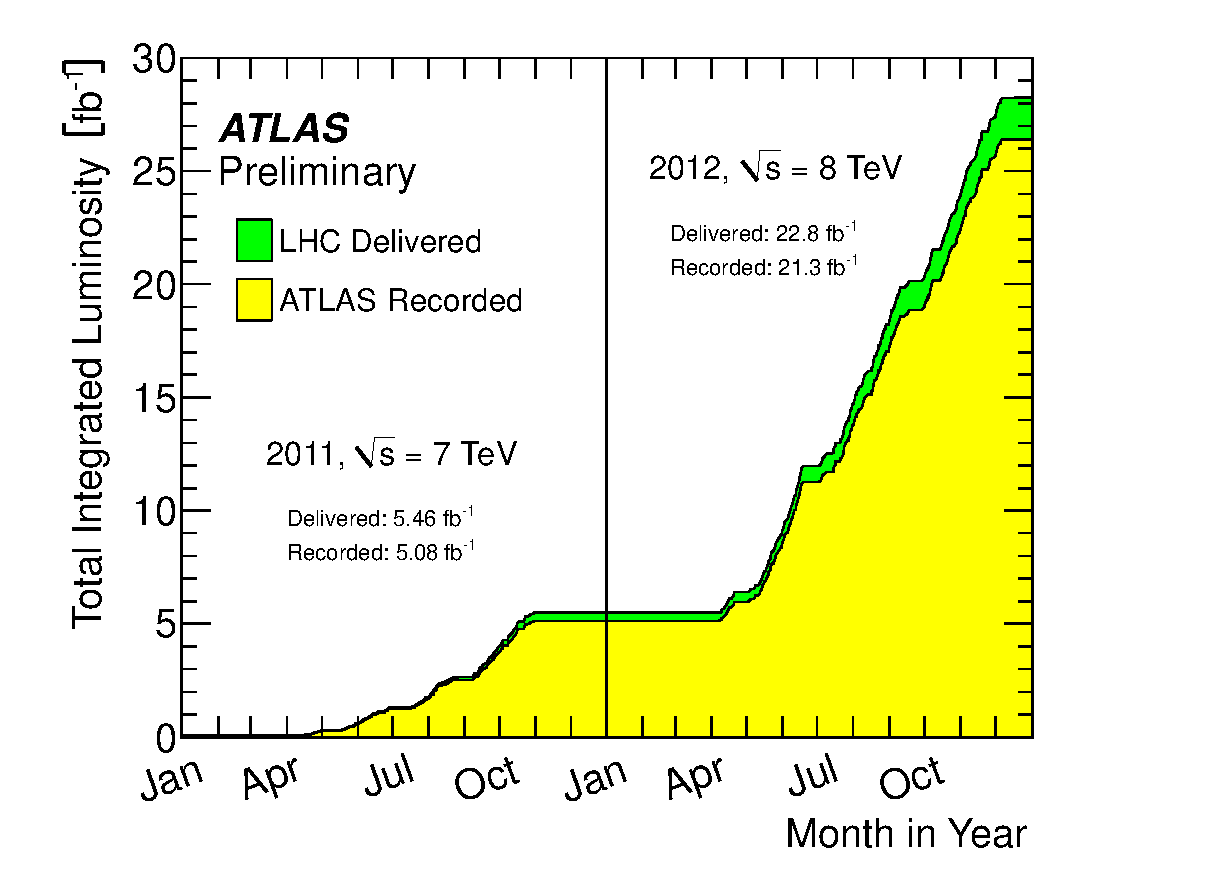
\includegraphics[width=\textwidth]{tex/experiment/luminosity}
		\caption{Luminosity}
		\label{fig:dataset:lumi}
	\end{subfigure}
	\hfill
	\begin{subfigure}[b]{0.495\textwidth}
		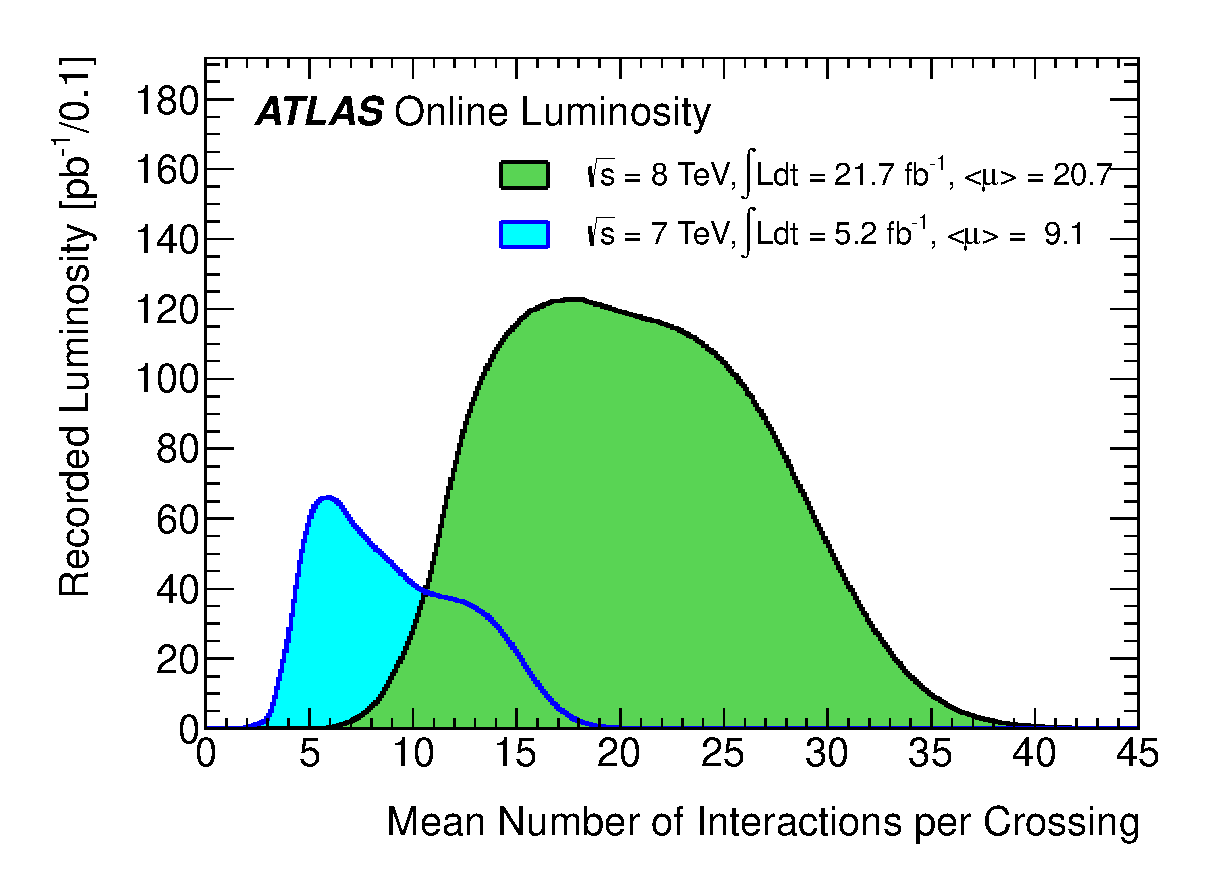
\includegraphics[width=\textwidth]{tex/experiment/pileup}
		\caption{Pile-up}
		\label{fig:dataset:pileup}
	\end{subfigure}
	\caption{(a) Cumulative luminosity delivered (green), recorded (yellow), and declared 
	`good for physics' (blue) during 2011 and 2012. Luminosities use the offline 
	calibration.
	(b) Mean number of interactions per bunch crossing $\mu$ for the 2011 (blue) and 
	2012 (green) datasets, calculated with an inelastic \pp cross section of 
	\unit{71.5}{\milli\barn} at \unit{$\sqrt{s} = 7$}{\TeV} and 
	\unit{73.0}{\milli\barn} at \unit{$\sqrt{s} = 8$}{\TeV}.
	Luminosities use the online calibration.}
	\label{fig:dataset}
\end{figure}

